%----------------------------------------------------------------------------------------
%----------------------------------------------------------------------------------------
%----------------------------------------------------------------------------------------
%DATA
%----------------------------------------------------------------------------------------
%----------------------------------------------------------------------------------------
%----------------------------------------------------------------------------------------

\section{Study sample}
\label{Sec: data_SOMN}

Our study includes 10 regions in M31 (Fig.~\ref{fig: regions in m31}) and 8 regions in M101 (Fig.~\ref{fig: regions in m101}). 
These specific regions were chosen for the availability of mid-infrared PAH spectroscopy.
Besides PAH line strnegths, for each galaxy, we use spectroscopic and photometric observations as well as their derived properties, such as SFR, stellar mass, dust luminosity (L$_{\rm dust}$) and mass, metallicity, and gas mass.
Table~\ref{tab: data} shows the full list of data and their units for both M31 and M101.
Observed values were divided by the area of their region (in arcsec$^2$), to remove the distance factor from the data and compare values across galaxies.
Since the spatial resolution of the observations varies from $<1\arcsec$ to $60\arcsec \times 90 \arcsec$, any attempt to match resolution would have caused a loss of information in some of the input quantities (e.g. the spectroscopic data).
In this project we used flux per unit area, which the convolution methods conserve~\citep{Aniano12}, as the input data.
Therefore, we did not perform any resolution matching and used data at their original resolution. %PB: Need to discuss these last few sentences; not sure I understand what you're saying.


\import{../sections/tables/}{tab_data.tex}

% \begin{figure}
%   \begin{subfigure}[b]{0.5\textwidth}
%         \centering
%     %\centering
%         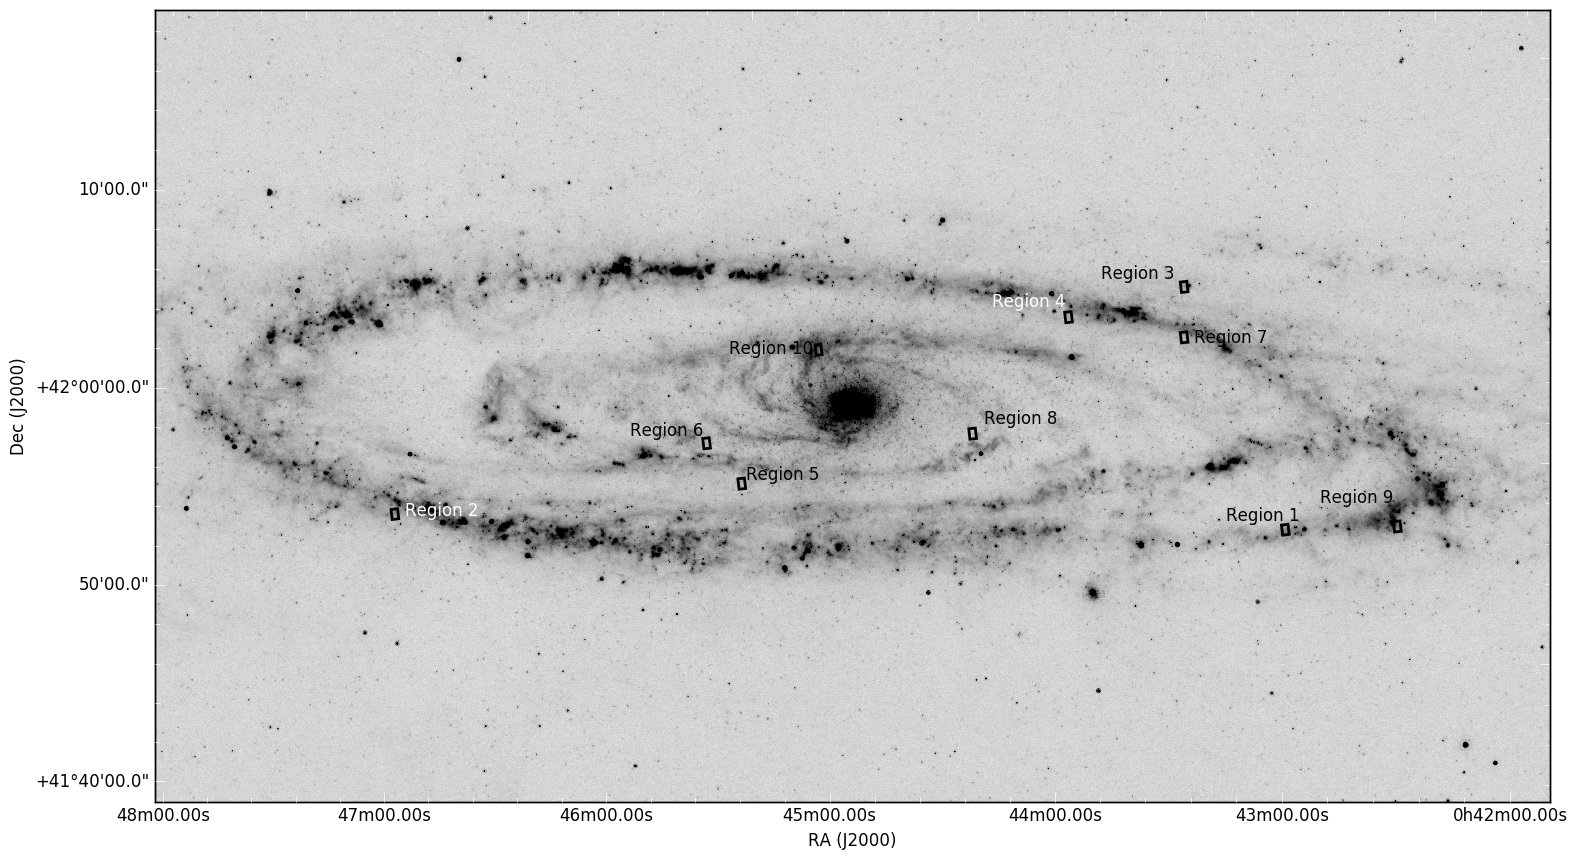
\includegraphics[width=0.97\textwidth]{../images0.0/M31/M31.png}
%         \caption{MIPS24 image of M31, with position of 10 regions that we studies.}
%         \label{fig: regions in m31}
%     \end{subfigure}
%     \hfill
%     \begin{subfigure}[b]{0.5\textwidth}
%         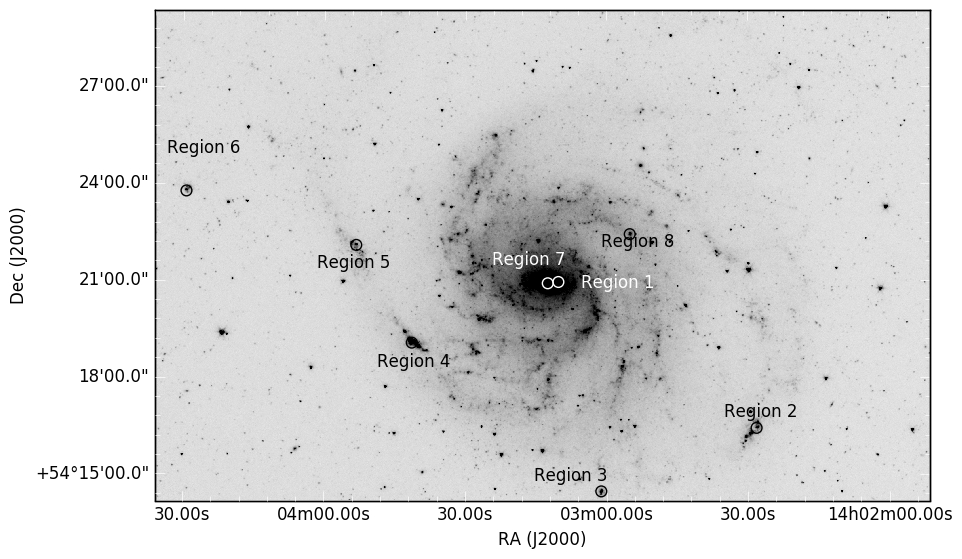
\includegraphics[width=\textwidth]{../images0.01/M101/M101.png}
%         \caption{IRAC1 image of M101, with position of our 8 regions that we studies.}
%     \label{fig: regions in m101}
%     \end{subfigure}
%     \caption{Position of the data in M31 (up) and M101 (down).}
% \end{figure}

  \begin{figure}
    \subfloat[MIPS 24~$\mu$m image of M31~\citep{Gordon06}, with position of 10 regions from~\cite{Dim15} \label{fig: regions in m31}]{
      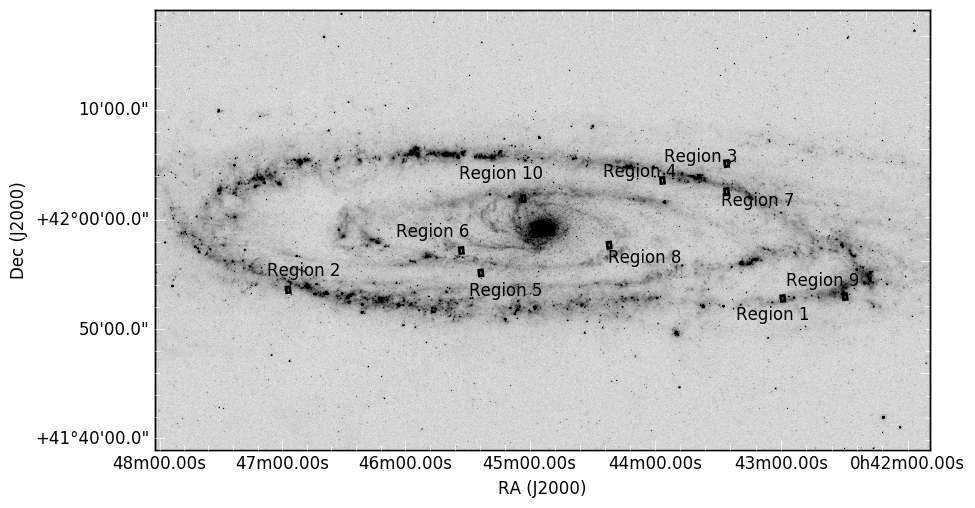
\includegraphics[width=0.5\textwidth]{../images0.01/M31/M31.png}
    }
    \hfill
    \subfloat[IRAC 3.6~$\mu$m image of M101~\citep{Dale09}, with position of 8 regions.\label{fig: regions in m101}]{
      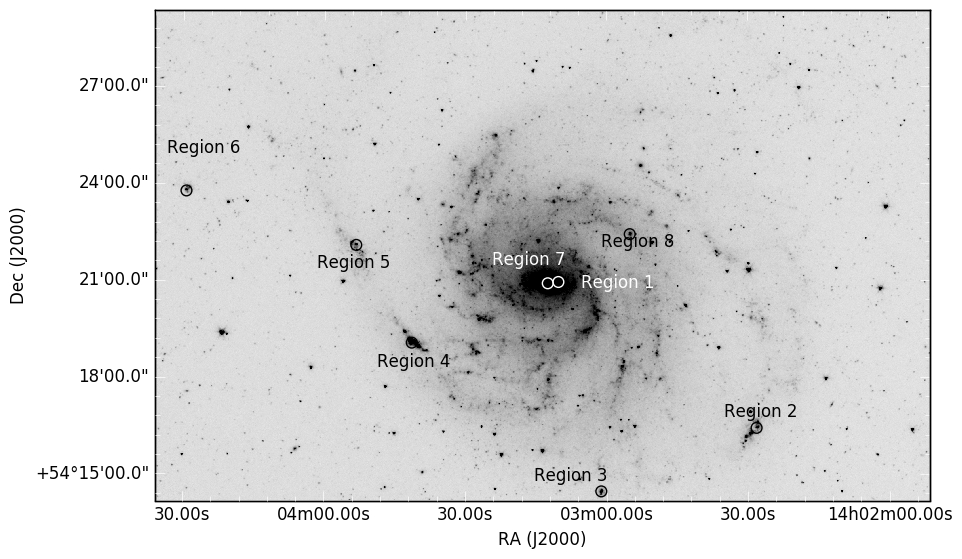
\includegraphics[width=0.5\textwidth]{../images0.01/M101/M101.png}}
    \caption{Position of regions that the input data for SOM that obtained from there in M31 (up) and M101 (down).}
    \label{fig:dummy}
  \end{figure}

%M31 data 
%%%%% Sahar: More detail, right?
    \subsection{M31 observations}
     \label{Sec: data_M31_SOMN} 
     
     %The 10 regions in M31 were chosen due to availability of the PAH data for them. 
     \cite{Dim15} using {\it Spitzer}/IRS observations to study PAHs in 10 regions chosen to span a range of mid-infrared flux ratios in M31. 
     Fluxes and equivalent widths of PAH and atomic line features were measured using the~{\sc PAHFIT IDL} tool~\citep{Smith07b}.
     %For spectroscopy part of our sample, we utilized their measured fluxes for PAH lines. 
     \cite{Dim15} also measured metallicity and radiation hardness index (RHI) for these 10 regions.
     We used the measured PAH feature fluxes, metallicity and RHI of each region as an input for SOMs.
     
    For the photometry part of the sample, we used the \GALEX~\citep{Martin05} far-ultraviolet and near-ultraviolet (FUV and NUV) channel images; \halpha, \sii~and \oiii narrow band images~\citep{Massey07}, IRAC 3.6, 4.5, 5.8 and 8.0$\mu$m images ~\citep{Barmby06}; MIPS24 and 70~$\mu$m~images\citep{Gordon06}; and PACS 100 and 160~$\mu$m and SPIRE 250, 350, and 500~$\mu$m~\citep{Fritz12} images.
     The units of all fluxes were converted to W~m$^{-2}$ in order to be the same as the PAH fluxes.
     $^{12}$CO (J:$1\rightarrow0$) line emission images~\citep{Nieten06} and atomic gas (H\,{\sc I}) 21~cm emission images from~\cite{Chemin09} were added to the input data. 
     For derived values, we utilized SFR(FUV + 24$\mu$m), stellar mass, molecular gas mass, atomic gas mass, total gas mass, and total infrared (TIR) luminosity (L$_{\rm TIR}$) from \cite{Rahmani16}, and L$_{\rm dust}$ and mass from \cite{Draine14}.
     
    \subsection{M101 observations}
    \label{Sec: data_M101_SOMN} 
     \cite{Gordon08} measured PAH fluxes, metallicity and RHI for M101 in XX regions chosen.. % PB: reason for selecting?
%     We also added their measurement of metallicity and RHI for these regions to our sample.
     We used NED~\footnote{The NASA/IPAC Extragalactic Database (NED) is operated by the Jet Propulsion Laboratory, California Institute of Technology, under contract with the National Aeronautics and Space Administration.} website to gather imaging observations of M101, including 
      \GALEX FUV and NUV~\citep{depaz07}, IRAC $3.6-8.0\mu$m, MIPS~24 and 70~$\mu$m~\citep{Dale09}, and  PACS~100 and 160~$\mu$m and SPIRE~250, 350, and 500~$\mu$m emission from~\cite{Kennicutt11}.
     As for M31, we used $^{12}$CO (J:$1\rightarrow0$) line emission images~\citep{Helfer03} and atomic gas (H\,{\sc I}) 21~cm emission images from \cite{Walter08}.
     SFR(FUV + 24$\mu$m), stellar and total gas mass maps were calculated using the same methods as for M31.
     
     Some of the correlations between single-wavelength emission and galaxy properties are well-known.
     Emission in the 3.6$\mu$m band traces the old stellar population very well~\citep[e.g]{Leitherer99,Smith07a} and it can be used to calculate the stellar mass~\citep{Eskew12}.
     FUV, \halpha, and TIR emission are indicators of star forming regions.
     In this project we used the SFR traced by the FUV emission, corrected for foreground stars using NUV emission and for dust extinction using 24$\mu$m emission.
     Total infrared emission is calculated from a modified version of~\cite{Draine07} calibration using using 8, 24, 70, and 160 $\mu$m emission~\citep{Boquien10}.
     To make sure that we do not use the observed data as input data in multiple forms, we removed all the observed data that were used to calculate galaxies properties from the input sample.
     We used this sample of observations as the main input for creating SOMs.
     Fig.~\ref{fig: cor_all} shows the Pearson correlation coefficients between the observations computed with a confidence level of $95\%$. 
     
     
      \begin{figure*}
                \centering
                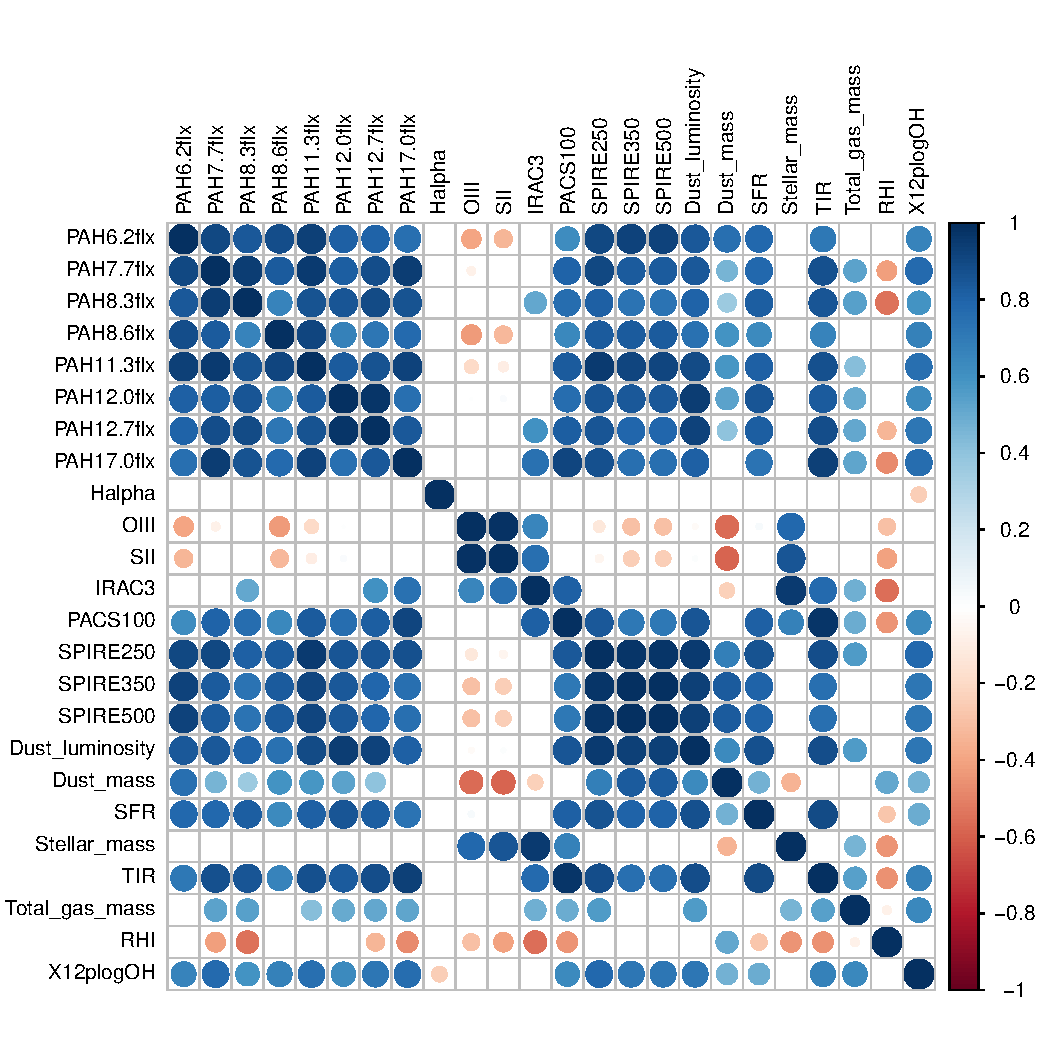
\includegraphics[width=\textwidth]{../images0.01/cor_plots/M31_all_derived_ones_core_plot_for_paper.pdf}
            \caption{Pearson correlation coefficients with a confidence level of 95$\%$ for all data in subset 0. The colours show the Pearson correlation coefficients where 1 means highly correlated and $-1$ means highly anti-correlated quantities. The non-significant correlations were left empty.}
            \label{fig: cor_all}
        \end{figure*}
 
  
